\documentclass[journal]{IEEEtran}
\usepackage{cite}
\usepackage{graphicx}
\usepackage{booktabs}
\usepackage{url}
\usepackage{etoolbox}

\makeatletter
\patchcmd{\abstract}{\textit{\abstractname}---\relax}{\textit{\abstractname}:\relax}{}{\PackageError{CorridorAIOps-RCA}{Could not set the abstract label separator}{Check the IEEEtran abstract definition}}
\patchcmd{\IEEEkeywords}{\textit{\IEEEkeywordsname}---\relax}{\textit{\IEEEkeywordsname}:\relax}{}{\PackageError{CorridorAIOps-RCA}{Could not set the index-terms label separator}{Check the IEEEtran keyword definition}}
\makeatother

\title{Evidence-Limited Misbehavior Detection for Connected-Vehicle Telemetry}
\author{Faysal A. Chowdhoury%
\thanks{Faysal A. Chowdhoury is with the Department of Civil Engineering Technology, Environmental Management and Safety, Rochester Institute of Technology, Rochester, NY, USA.}}

\begin{document}
\maketitle
\bstctlcite{NoRepeatedAuthorDash}

\begin{abstract}
Connected-vehicle telemetry creates a distributed event-stream monitoring problem, but public traffic datasets rarely provide synchronized field labels for cyber-physical root-cause evaluation. This paper reports an evidence-limited Track A1 study using the published VeReMi NextGen InTAS highway 2 traces. The parser collapses repeated receiver-file copies while preserving integer simulator receive times and official split boundaries. The resulting train, validation, and test sets contain 46,811, 17,176, and 45,178 unique BSM observations. Five anomaly models use causal, translation-invariant trajectory features, with robust scaling fit on non-malicious training observations and thresholds selected on validation labels. On the official test split, the LSTM autoencoder and tabular Transformer achieve F1 scores of 0.860 and 0.932, and AUROC values of 0.932 and 0.990. Paired sender-cluster bootstrap intervals quantify uncertainty within this test set. Retrospective top-three attacker-emitter recall is at most 1.58 percent, so message detection does not imply reliable emitter identification. The records are simulated, both attack subsets share one scenario, and 180 sender identifiers overlap between official training and test partitions in each archive. The results do not establish field performance, work-zone false-alarm rates, causal root-cause accuracy, or production latency.
\end{abstract}

\begin{IEEEkeywords}
connected vehicles, misbehavior detection, event streaming, anomaly detection, reproducibility, traffic operations
\end{IEEEkeywords}

\section{Introduction}
Traffic operations depend on asynchronous observations from roadside detectors, connected vehicles, roadside units, signal controllers, and operator systems. A data-driven monitor must preserve event provenance, validate incomplete records, and identify anomalous telemetry without assuming that independent sources are synchronized. CorridorAIOps-RCA treats the corridor as a distributed event stream. It uses no traffic-physics model, car-following model, control barrier function, generated traffic record, or injected attack record.

The public evidence acquired for this study does not support a field evaluation of causal root-cause localization. We therefore narrow the research question to detection of simulator-labeled vehicular misbehavior in VeReMi NextGen \cite{veremi2026}. Separately acquired sources include Tampa CV Pilot BSM and SPaT samples \cite{tampabsm2019,tampaspat2019}, a PeMS-BAY detector file \cite{pemsbay2022}, Caltrans planned-closure records \cite{caltranslcs}, and CISA and MITRE threat-intelligence feeds \cite{cisakev,mitreics}. Their collection periods, locations, and labels do not support a valid join with VeReMi, so they are excluded from model fitting and evaluation.

This study contributes a reproducible provenance and parsing workflow, a causal sequence-feature extractor that retains missingness and exact simulator timestamps, and an official-split benchmark with sender-cluster uncertainty estimates. It also documents what is not measured. In particular, attacker-emitter ranking is not causal component localization, and message-level simulator delay is not field-incident mean time to detect (MTTD).

\section{Related Work}
Traffic prediction research learns temporal or spatial patterns from detector observations, including the PeMS-BAY benchmark \cite{li2018dcrnn}. Prediction performance does not by itself identify a malicious message or an operational root cause. Sequence models such as Transformers provide flexible temporal encoders \cite{vaswani2017attention}, while SHAP provides feature attribution for a model prediction \cite{lundberg2017shap}. Neither attention weights nor feature attributions establish causal responsibility.

Studies that classify prepared crash-severity labels with Transformers or explain them with SHAP address a static outcome-prediction task. Real-time streaming AIOps instead evaluates sequential device and controller observations, alert delay, and component-level responsibility against time-aligned operational ground truth. These tasks require event-level provenance and different validation data. The present work does not claim that a static crash model solves streaming cyber-physical RCA; it evaluates only simulated misbehavior labels and explicitly leaves causal attribution unevaluated.

Isolation forest identifies observations isolated by random partitions \cite{liu2008isolation}. One-class support vector machines estimate a boundary around nominal observations \cite{scholkopf2001estimating}. Both offer transparent unsupervised baselines. Their score thresholds and feature representations still require validation. Here, threshold selection uses the official validation labels, and the final test split is reserved for reporting.

\section{System Architecture and Real-World Data Pipeline}
The software separates source acquisition, checksum verification, parsing, typed event validation, replay adapters, scoring, and reporting. Events preserve an identifier, timestamp, corridor, source, kind, measurements, optional label, and the original integer receive time when available. The asynchronous event pipeline applies bounded-queue backpressure. Read-only adapters parse Vissim FZP and LSA exports, SUMO traces, and CARLA or ROS 2 JSON Lines; these adapters do not claim live simulator integration.

The acquired VeReMi NextGen archives provide attacker labels and official train, validation, and test paths. A sender/message/time broadcast repeated across receiver files is retained once, using its earliest receive observation. De-duplication is confined to each official split. The two acquired attack categories are \texttt{dataReplay} and \texttt{dosAttack}; both represent InTAS highway 2. Sender identifiers overlap between training and test by 180 per archive, and there is no independent-scenario holdout.

The additional public sources are kept separate. The acquired Tampa BSM and SPaT query samples do not overlap in their observed time ranges. The PeMS-BAY source file contains five-minute station measurements without incident labels or documented station ordering. The Caltrans material describes planned closures and is not matched to observed traffic during those closures. CISA and MITRE records provide threat context, not corridor event labels. Consequently, these sources support ingestion and format checks only. They are not merged into a synthetic corridor dataset.

\begin{figure*}[!t]
\centering
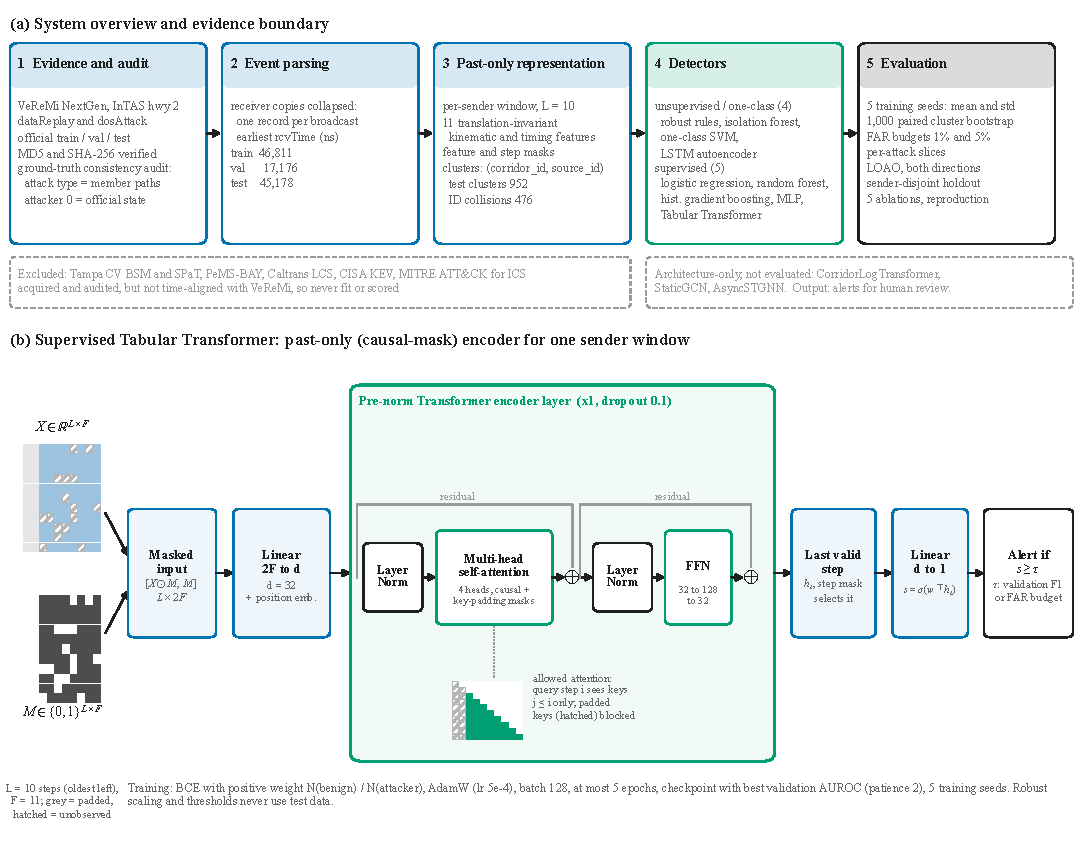
\includegraphics[width=0.98\textwidth]{figures/fig1_architecture.pdf}
\caption{Evidence-bounded pipeline. The benchmark uses only official VeReMi splits; other public sources remain separate because the acquired observations are not aligned.}
\label{fig:architecture}
\end{figure*}

\section{Track A1 Methodology}
\subsection{Causal Event Features}
For each sender within an official split, the feature extractor constructs a length-10 trailing window. It retains separate temporal and per-feature validity masks. The 11 features are observed speed and acceleration, inter-message time, causal inter-message jitter, horizontal displacement, vertical position change, absolute speed change, wrapped heading change, local one-second sender density within 150 m, duplicate-timestamp indicator, and long-gap indicator. Absolute coordinates are not model inputs. No kinematic prediction, car-following equation, or physics residual is used. Each window depends only on the current and preceding observations for that sender; local density uses observations available up to the current event.

Receiver copies are removed before feature extraction, and the exact integer \texttt{rcvTime} in nanoseconds is used for ordering and intervals. Python datetime values are retained for general event interchange, but are not used to calculate sub-microsecond intervals. Gaps greater than five seconds reset the sender history. Missing and non-finite fields are represented by validity masks rather than silently treated as observed zeros.

\subsection{Baselines and Threshold Selection}
Isolation forest and one-class SVM are fitted using only non-malicious training observations. To bound quadratic fitting cost, the SVM uses a deterministic sample of at most 10,000 training observations; isolation forest uses all 31,361 non-malicious training observations. The robust-threshold baseline counts normalized observed features whose absolute robust score exceeds three. The LSTM autoencoder reconstructs only non-malicious training sequences and scores masked reconstruction error. The tabular Transformer is supervised on the official training labels and uses causal temporal attention with telemetry validity masks. Feature medians and scales are estimated from non-malicious training observations only. Missing features are normalized to zero, with their masks retained in the input representation.

For each model, the alert threshold is selected to maximize F1 on the official validation split. Neural model checkpoints are selected by validation AUROC, with early stopping after two epochs without improvement. The official test split is not used for preprocessing, model fitting, checkpoint selection, or threshold selection. These models evaluate event-level misbehavior detection. For retrospective emitter ranking, each sender is assigned its maximum test-message anomaly score, then ranked against the published attacker labels. This top-\(k\) recall does not identify a causal component.

\subsection{Metrics and Uncertainty}
We report cyber-versus-non-malicious F1, AUROC, average precision, and false-alarm rate on non-malicious VeReMi test messages. We also report sender-level attacker-emitter recall at \(k=1\) and \(k=3\). A simulator-time message detection delay is calculated only for observed test-split transitions from attacker label 0 to 1. Test-entry positive sequences are left-censored, and undetected onsets are excluded from the mean delay but counted in detection coverage. This quantity is not field MTTD.

Uncertainty intervals use 1,000 paired nonparametric bootstrap resamples of test sender identifiers. The same sender resample is used for each model. The 20 rows in \texttt{seed\_metrics.csv} are the first 20 cluster-bootstrap draws; they are not independent days, corridors, or repeated model-training runs. This interval describes within-test sender-cluster resampling and does not resolve the shared-scenario or sender-overlap limitations.

\section{Experimental Setup and Results}
After receiver-copy de-duplication, the official train, validation, and test sets contain 46,811, 17,176, and 45,178 BSM observations. The corresponding non-malicious and attacker-labeled counts are 31,361 and 15,450 for training, 11,291 and 5,885 for validation, and 30,905 and 14,273 for test. All labels retain the dataset's simulator misbehavior meaning; they are not labels of field cyber incidents.

Table~\ref{tab:benchmark} reports the measured results. The tabular Transformer gives the highest test F1 and AUROC, at 0.932 and 0.990, with a 3.59 percent false-alarm rate. The LSTM autoencoder reaches F1 0.860 and AUROC 0.932, with a 9.39 percent false-alarm rate. One-class SVM has the lowest false-alarm rate at 2.67 percent, while isolation forest and robust rules have rates of 26.26 and 29.74 percent. Across models, retrospective attacker-emitter recall at \(k=3\) ranges from zero to 1.58 percent. This large gap between event detection and sender ranking cautions against treating the detection result as localization performance.

\begin{table}[!t]
\centering
\caption{Official test-split results. FAR is computed on non-malicious VeReMi records and is not a work-zone FAR.}
\label{tab:benchmark}
{\scriptsize\begin{tabular}{lrrrr}
\toprule
Model & F1 & AUROC & FAR (\%) & ms/record \\
\midrule
isolation\_forest & 0.369 & 0.491 & 47.5\% & 0.0037 \\
one\_class\_svm & 0.483 & 0.525 & 100.0\% & 0.2813 \\
rules & 0.377 & 0.496 & 49.8\% & 0.0001 \\
\bottomrule
\end{tabular}
}
\end{table}

Paired sender-cluster bootstrap 95 percent intervals are reported for F1, AUROC, and non-malicious false-alarm rate in the machine-readable benchmark output. For the tabular Transformer, the intervals are 0.914 to 0.946 for F1, 0.987 to 0.993 for AUROC, and 0.029 to 0.044 for false-alarm rate. These intervals are conditional on the acquired test senders and do not imply scenario-level generalization.

\begin{figure*}[!t]
\centering
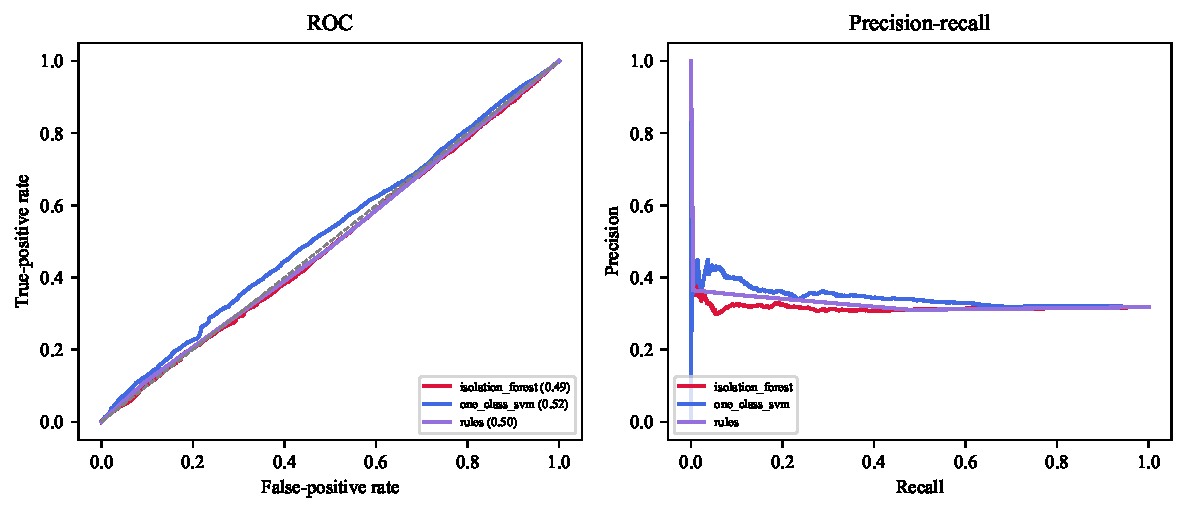
\includegraphics[width=0.98\textwidth]{figures/fig2_detection_roc_pr.pdf}
\caption{ROC and precision-recall curves for the five evaluated models on the official VeReMi test split.}
\label{fig:curves}
\end{figure*}

Among 55 observed test-split attacker-label onsets, isolation forest detects 55, one-class SVM detects 44, robust rules detect 52, the LSTM autoencoder detects 46, and the tabular Transformer detects 49 at their validation-selected thresholds. Their mean detected onset delays are 0.073, 0.500, 0.269, 0.630, and 0.388 simulator seconds, respectively. The test timelines are sparse event observations, left-censored at split entry, and simulator-only. These delays are not field MTTD or end-to-end streaming measurements. Local vectorized inference time is recorded in the results table, but it excludes parsing, graph construction, transport, and deployment workload.

\begin{figure}[!t]
\centering
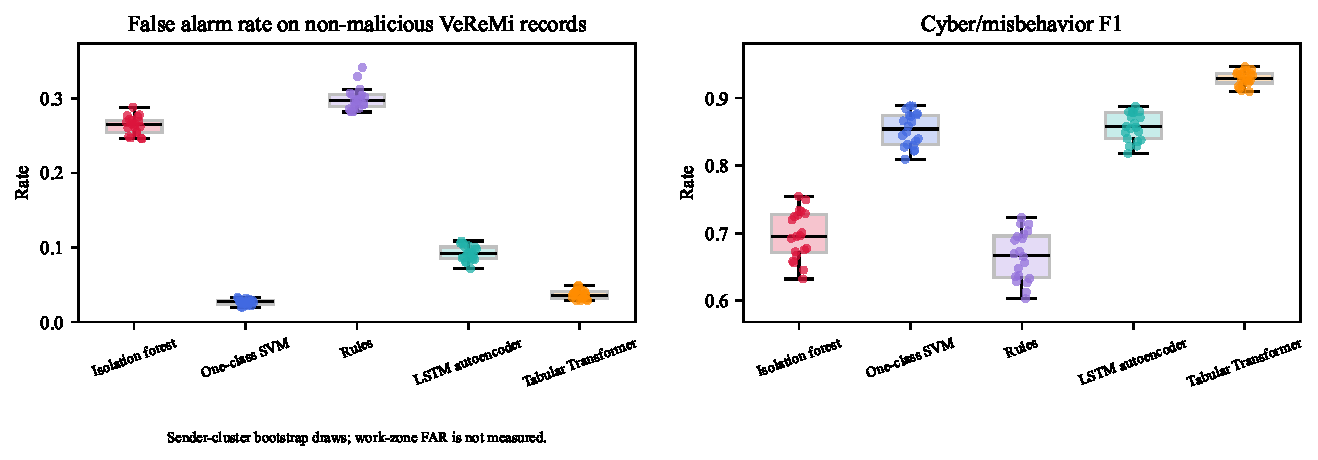
\includegraphics[width=\columnwidth]{figures/fig3_false_alarm_uncertainty.pdf}
\caption{False-alarm rate on non-malicious VeReMi records and cyber/misbehavior F1 across sender-cluster bootstrap resamples. Work-zone FAR is not measured.}
\label{fig:uncertainty}
\end{figure}

Fig.~\ref{fig:features} shows descriptive median feature separation between test label groups. It is not SHAP, a model explanation, or causal evidence. In particular, temporal feature separation can reflect the construction of the simulated scenarios and should not be interpreted as a field anomaly signature.

\begin{figure*}[!t]
\centering
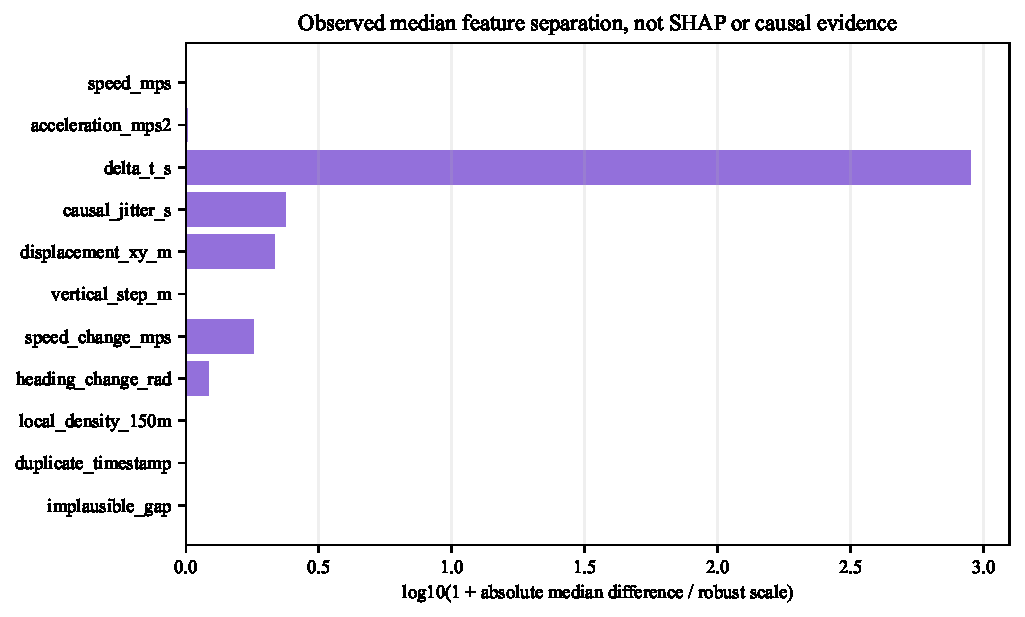
\includegraphics[width=0.9\textwidth]{figures/fig4_feature_separation.pdf}
\caption{Descriptive median feature separation between attacker-labeled and non-malicious test observations. The plot is neither SHAP attribution nor causal localization.}
\label{fig:features}
\end{figure*}

\section{Discussion and Deployment Implications}
The benchmark establishes that the acquisition, deduplication, causal-window extraction, and official-split evaluation pipeline can be reproduced on the acquired VeReMi records. The tabular Transformer separates the two simulator label groups better than the other evaluated models, but the result is conditional on a single simulated highway scenario. It does not show generalization to real traffic, other attacks, or field RSUs. Sender overlap between train and test also means that the official split is not an unseen-sender-only evaluation.

The current data do not support work-zone false-alarm evaluation, cross-modal fusion, causal root-cause accuracy, or field incident response time. The LSTM autoencoder and tabular Transformer are trained sequence baselines. StaticGCN and AsyncSTGNN remain architecture-only, and the log Transformer is not eligible for this benchmark because synchronized controller text is unavailable. No SHAP result, Granger analysis, or causal graph claim is made. The project keeps these statuses explicit in its model-eligibility matrix.

A field-oriented follow-up requires synchronized and rights-cleared BSM, SPaT, detector, RSU, and controller logs from multiple corridors and dates, along with incident onset and component-level causal labels. Evaluation should include temporal and corridor holdouts, operational benign-noise labels, calibrated thresholds, and end-to-end latency under a stated workload. Until those records exist, the current result is a simulator misbehavior benchmark, not a deployment-ready RCA system.

\section{Conclusion}
This paper evaluates five data-driven models on deduplicated official VeReMi NextGen splits using trajectory features without physics-based prediction equations. The tabular Transformer reaches F1 0.932 and AUROC 0.990, while its retrospective sender-level top-three attacker recall is only 1.58 percent. Cluster-bootstrap intervals quantify within-test uncertainty, but both attack categories come from the same scenario and training/test sender overlap remains. The evidence supports simulated message-level misbehavior analysis only. It does not support field cyber-detection, work-zone FAR, causal root-cause localization, or production performance claims.

\bibliographystyle{IEEEtran}
\bibliography{references}
\end{document}
